\usetikzlibrary{shapes.geometric}
\usetikzlibrary{positioning}

\newcommand{\apparatus}[4]{\node[square node] (#1) at (#2,#3){#4};
                           \node[port] (#1+) at (#2 + 0.375, #3 + 0.5){+};
                           \node[port] (#1-) at (#2 + 0.375, #3 - 0.5){-};}

\chapter{Postulates of Quantum Mechanics}

We first consider the mathematical objects used to model physical systems and variables. By comparing the objects used in classical and quantum mechanics, we make sense of the first three postulates of quantum mechanics. Then, we compare the Copenhagen and von Neumann descriptions of measurement and their relation to the fourth and fifth postulates.

\section{Physical Variables and State Spaces}
\subsection{Classical States}
Consider the spin of an electron. Treating the electron as a classical system, its spin state is modeled by a vector $\vec{S} \in \mathbb{R}^3$:
\begin{align}
\vec{S} = (S_x, S_y, S_z)
\end{align}

Each component $S_{x_i}$ is a physical variable representing the magnitude of spin oriented in the $\hat{x_i}$ direction.

$\vec{S}$ has the capacity to determine spin in any direction using the inner product of the state space $\mathbb{R}^3$:
\begin{align}
S_n(S) = \vec{S} \cdot \hat{n}
\end{align}

We see that in classical mechanics, physical variables are modeled using functions. Each function $S_n$ maps a spin state $[\vec{S}$ to a real scalar representing the spin of the electron aligned along the $\hat{n}$ axis.

What makes classial mechanics familiar to everyday experience boils down to intuitive but important properties of the state space $\mathbb{R}^3$:
\begin{itemize}
\item For any direction $\hat{n}$, $\vec{S}$ determines spin $S_n$
\item $S_n$ can be any real value
\end{itemize}

$\vec{S}$ determines spin in any direction because TODO. Consequently, the sample spaces for spin in any two directions $\hat{n}$ and $\hat{m}$ are \textit{compatible}, meaning that $S_n$ and $S_m$ may be simultaneously determined. Spin states in $\mathbb{R}^3$ are interpreted physically as the electron posessing definite values for every $S_n$ at some instant in time.

In addition to spin states determing all $S_n$, the state space allows $S_n$ to take on any real value. There are no fundamental restrictions on which real numbers $S_n$ could be; its sample space is continuous and infinitely large.

\subsection{Quantum States}
Measurements of electron spin show that the intuitive classical properties do not hold. Recall that only two magnitudes of spin have ever been measured. $S_n$ is a \textit{quantized} physical variable; its sample space is discrete and finite.

Second, the results of successive measurements of a spin system imply that $\vec{S}$ does not determine spin in some general direction $S_n$. Recall the results of succesively measuring spin in orthogonal directions discussed in TODO REF. After measuring $S_x$, $\vec{S}$ appears to ``forget'' a previous measurement of $S_z$. All we may know about the system at one instant in time is spin in one direction. The inabilitiy to simultaneously determine spin in two independent directions $\hat{n}$, $\hat{m}$ should be reflected through $S_n$ and $S_m$ having \textit{incompatible} sample spaces.

Electron spin measurements violate the intuitive classical state space properties mentioned in 3.1.1. In response, we must change the mathematical objects used to represent system states and physical variables. Specifically, the sample space of $S_n$ must restrict observable values to spin up and spin down, and $S_n$ and $S_m$ should have incompatible sample spaces. In combination, the first three postulates of quantum mechanics take care of these differences.

Quantum mechanics postulates that a system's state is completely described by a normalized vector in a linear state space.

\invisiblesubsubsection{Postulate 1 (System States)}
\begin{Thm:Postulate}{1}
    The state of a physical system is defined by specifying an abstract vector $\ket{\psi}$ in a Hilbert state space $\mathcal{H}$.
\end{Thm:Postulate}

For spin-$\frac{1}{2}$ systems such as electrons, the two-dimensional Hilbert space consists of all linear combinations of spin-up and spin-down:
\begin{equation}
  \ket{\psi} \in \mathcal{H} \\ \nonumber
  \ket{\psi}\{\alpha\ket{+} + \beta\ket{-}\}
\end{equation}
where $\alpha, \beta \in \mathbb{C}$.

$\mathcal{H}$ is an abstract state space; components of $\ket{\psi}$ cannot be interpreted as physical variables as they are for the classical spin state $S$. So, we introduce physical meaning with more postulates.

\invisiblesubsubsection{Postulate 2 (Physical Variables as Operators)}
The second posulate of quantum mechanics states that physical variables are described by linear operators:
\begin{Thm:Postulate}{2}
    Every physical variable $\mathcal{A}$ is described by an operator $A$ acting in $\mathcal{H}$.
\end{Thm:Postulate}

\invisiblesubsubsection{Postulate 3 (Observable Values)}
Justifying the second postulate is easiest when also considering the third postulate:
\begin{Thm:Postulate}{3}
    The only possible result of the measurement of a physical variable $\mathcal{A}$ is one of the eigenvalues of the corresponding operator $A$.
\end{Thm:Postulate}

The operator correlates elements of a finite sample space (eigenvalues) with particular system states (eigenstates). Consequently, a state can only be interpreted as having a definite variable value if it is an eigenstate of that variable's operator. To illustrate this, consider the operator representing $S_z$. Written in the basis of its own eigenstates,
\begin{align}
    S_z \doteq \frac{\hbar}{2}\begin{bmatrix} 1 & 0 \\ 0 & -1 \end{bmatrix}
\end{align}
This operator correlates $z$ spin-up $\left(S_z = \frac{\hbar}{2}\right)$ with eigenstate
\begin{align}
    \ket{\psi} = \ket{+_z} \doteq \begin{bmatrix} 1 \\ 0 \end{bmatrix}
\end{align}
and $z$ spin-down $\left(S_z = \frac{-\hbar}{2}\right)$ with eigenstate
\begin{align}
    \ket{\psi} = \ket{-_z} \doteq \begin{bmatrix} 0 \\ 1 \end{bmatrix}
\end{align}
Here, the subscript $z$ specifies that the state represents spin-up along the $z$ axis.

Similarly, we write the operator representing $S_x$ in the $S_z$ basis:
\begin{align}
        S_x \doteq \frac{\hbar}{2}\begin{bmatrix} 0 & 1 \\ 1 & 0 \end{bmatrix}
\end{align}
This operator correlates $x$ spin-up $\left(S_x = \frac{\hbar}{2}\right)$ with eigenstate
\begin{align}
    \ket{\psi} = \ket{+_x} \doteq \frac{1}{\sqrt{2}}\begin{bmatrix} 1 \\ 1 \end{bmatrix}
\end{align}
and $x$ spin-down $\left(S_x = \frac{-\hbar}{2}\right)$ with eigenstate
\begin{align}
    \ket{\psi} = \ket{-_x} \doteq \frac{1}{\sqrt{2}}\begin{bmatrix} 1 \\ -1 \end{bmatrix}
\end{align}

Operators for $S_z$ and $S_x$ share no common eigenstates, so no state can posses definite values for both variables. In general, operators for any two spin components $S_i$ and $S_j$ do not share common eigenstates with each other; in other words, $S_i$ and $S_j$ have incompatible sample spaces. $S_i$ and $S_j$ are called \textit{complementary} variables.

By representing physical variables with operators rather than functions, sample spaces become quantized and may be incompatible with each other. These features are necessary for predicting the results of electron spin measurements.

The first three postulates designate the mathematical objects used to model physical system states and variables. The fundamental differences between classical and quantum systems are completely described by these postulates and their consequences.

\subsection{Linearity}
TODO: compare addition of $S_x, S_y$ states and their interpretations. Introduce superposition states and coherence.

\section{Copenhagen Description of Measurement}
The fourth and fifth postulates constitute the Copenhagen description of measurement. This description, taught in textbooks and introductory quantum courses, is a key component of the standard interpretation of quantum mechanics.

The probability postulate, also known as the \textit{Born Rule}, assigns a probability distribution to the sample space of a physical variable.

\invisiblesubsection{Postulate 4 (Probability Distribution of Measurement Outcomes)}
\begin{Thm:Postulate}{4}
    When measuring physical variable $A$, the probability $\mathcal{P}(n)$ of obtaining result $a_n$ corresponding to $\ket{a_n}$  is equal to
     \begin{align}
        \mathcal{P}(n) = |\braket{a_n|\psi}|^2
    \end{align}
\end{Thm:Postulate}

The probabilities assigned to each state leaving the $S_x$ Stern-Gerlach device in Figure \fref{Figure:Measurement:DetectorStates} are
\begin{align}
    \mathcal{P}(+_y) &= |\braket{+_x|+_z}|^2 = \frac{1}{2} \\
    \mathcal{P}(-_y) &= |\braket{-_x|+_z}|^2 = \frac{1}{2}
\end{align}

The spirit of the Born Rule is unchanged in consistent quantum theory. Differences are discussed in (TODO: ref future section).

\invisiblesubsection{Postulate 5 (Collapse Dynamics)}

The fifth postualte (known as the projection postulate) describes how a system evolves upon measurement. Contingent upon interaction of the system with a ``classical apparatus'', measurement instantaneously changes the state of the system to some eigenstate of the variable being measured.

\begin{Thm:Postulate}{5} \label{projection postulate}
    If the measurement of the physical variable $\mathcal{A}$ on the system in the state $\ket{\psi}$ gives the result $a_n$, the state of the system immediately after the measurement is the normalized projection
    \begin{align}
        \ket{\psi^\prime} = \frac{P_n\ket{\psi}}{\sqrt{\bra{\psi}P_n\ket{\psi}
        }}
    \end{align}
    onto the subspace associated with $a_n$.
\end{Thm:Postulate}

Consider a measurement result for the $z$ component of spin. We represent the result with $n_z$, which could be either spin-up $\left(+_z \right)$ or spin-down $\left(-_z \right)$. The new state is the normalized projection of $\ket{\psi}$ onto $\ket{n_z}$. In other words, $\ket{\psi}$ instantaneously becomes $\ket{n_z}$ upon measurement. This process is known as \textit{state collapse} or \textit{wavefunction collapse}.

\begin{figure}
\centering\CaptionFontSize
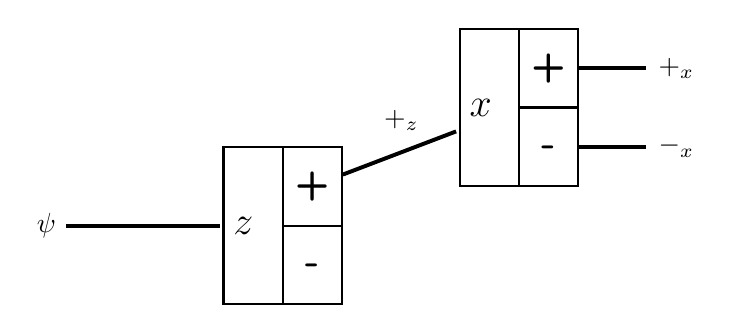
\begin{tikzpicture}[shorten >=1pt,auto, thick,
     square node/.style={rectangle, minimum height=2cm, minimum width=1.50cm, text width = 1.25cm, draw, font=\sffamily\Large\bfseries},
     port/.style={rectangle, draw,  minimum height=1cm, minimum width=0.75cm, font=\sffamily\Large\bfseries},
     wf/.style={rectangle, minimum height=1cm}]
    \apparatus{1}{3}{0}{$z$};
    \apparatus{2}{6}{1.5}{$x$};

    \node[wf] (w0) at (0,0) {$\ket{\psi}$};
    \node[wf] (w1) at (8, 2.0) {$\ket{+_x}$};
    \node[wf] (w2) at (8, 1.0) {$\ket{-_x}$};

    \draw[line width=0.5mm] (w0) -- (1);

    \draw[line width=0.5mm] (1+) -- (2) node [near end] {$\ket{+_z}$};

    \draw[line width=0.5mm] (2+) -- (w1);
    \draw[line width=0.5mm] (2-) -- (w2);
\end{tikzpicture}
\caption[Insert an abbreviated caption here to show in the List of Figures]
{The Stern-Gerlach experiment as described by the standard measurement scheme. Notice that each measurement outcome is renormalized, so that information about the state prior to measurement is lost.}
\label{Figure:Measurement:Renormalizing}
\end{figure}

\subsection{Example 1}

As an example, consider the Stern-Gerlach experiment shown in \fref{Figure:Measurement:Renormalizing}. The first apparatus serves as a state preparation device, since we are only interested in particles exiting the spin-up output. Using the projection postulate, the state after the first measurement is
\begin{align}
    \ket{\psi^\prime} &= \frac{{P^z_+}\ket{\psi}}{\sqrt{\bra{\psi}P^z_+\ket{\psi}}} = \ket{+_z}
\end{align}
Similarly, the possible output states from the second apparatus are
\begin{align}
  \ket{\psi^{\prime\prime}} &= \frac{P^x_+\ket{+_z}}{\sqrt{\bra{+_z}P^x_+\ket{+_z}}} = \ket{+_x}
\end{align}
or
\begin{align}
  \ket{\psi^{\prime\prime}} &= \frac{P^x_-\ket{+_z}}{\sqrt{\bra{+_z}P^x_-\ket{+_z}}} = \ket{-_x}
\end{align}

\section{Dynamics}
In a mechanical theory, the equations of motion (or \textit{dynamics}) describe how a state evolves with time. In classical Newtonian mechanics, this is given by Newton's law of motion
\begin{align}
  \vec{F} = m\vec{a}.
\end{align}

These dynamics are \textit{unitary}, meaning that given the final state of a physical process, the corresponding initial state is recovered by applying the dynamics with time reversed. The dynamics can be represented by a one-to-one map from initial to final states.

The projection postulate describes one type of dynamics, which apply only during measurement. When applied, all information about the initial state is lost as the state instantaneously becomes an eigenstate of the measured variable. The map from initial to final states is not one-to-one; ``collapse dynamics'' are non-unitary.

Quantum theory postulates an another type of dynamics that is analogous to Newton's law of motion. These dynamics are unitary, and apply at all times (not just during measurement).

\invisiblesubsubsection{Postulate 6 (Unitary Dynamics)}
\begin{Thm:Postulate}{6}
  TODO write Schrödinger equation
\end{Thm:Postulate}

\chapter{Measurement}

TODO: chapter preview
State collapse requires extra assumption, ambiguous defs lead to interepretation issues, arrow of time

\section{Issues with State Collapse}

The projection postulate introduces foundational assumptions to describe the measurement process. The principle of Occam's razor says that, in general, a theory is strengthened by making as few assumptions as possible. In classical mechanics, there are no foundational assumptions made to describe measurement; this motivates the pursuit to describe quantum measurement without using the projection postulate.

Furthermore, the projection postulate relies on ambiguous definitions. State collapse occurs upon ``interaction with a classical measuring apparatus'', yet there is no specification of what makes a system classical. Classical systems are not described by the theory, yet they play a fundamental role in the measurement process.

TODO: describe interpretational issues

% This ambiguity makes quantum mechanics exploitable for justification of anthropocentric statements. Examples are widespread in both popular and scientific literature. In the 1975 bestseller \textit{The Tao of Physics},
% \begin{quote}
%  ``The human observer constitutes the final link in the chain of observational processes, and the properties of any atomic object can only be understood in terms of the object's interaction with the observer.'' \cite{Capra}
% \end{quote}
% Similarly, the von Neumann-Wigner interpretation of quantum mechanics asserts that
% \begin{quote}
%  ``[t]here exist external observers which cannot be treated within quantum mechanics, namely human (and perhaps animal) minds, which perform measurements on the brain causing wave function collapse.'' (Schreiber's description of the von Neumann–Wigner interpretation \cite{Schreiber}).
% \end{quote}
%
% This attitude towards quantum measurement prompted Einstein to ask a colleague if they believed that the moon existed only when they looked at it \cite{Pais}. In this thesis, we assert that the moon does exist, even when not directly observed by a human. Instead, we allow a multitude of non-living systems to continuously ``measure'' the moon. This is done using the \textit{von Neumann measurement scheme}, which describes measurement as a physical process involving two quatum systems, neither of which need be human or a ``classical measuring apparatus''.

Because the measurement process cannot be reversed, state collapse injects time asymmetry into the foundations of quantum mechanics. TODO: discuss arrow of time.

The issues with interpretation of state collapse and non-unitary dynamics in general are indicators that collapse dynamics are formulated with ignorance of some underlying process. To begin describing this process, we discard the projection postulate and describe measurement using dynamics permitted by the Schrödinger equation.

Describing measurement as a unitary process is desirable for multiple reasons:
\begin{itemize}
  \item With dynamics symmetric in time, the emergence of the ``arrow of time'' can be studied
  \item Humans and measurement apparatuses do not play a special role indescribale by the theory
  \item TODO: describe cosmology benefit.
  \item interpretational issues with state collapse go away
  \item less fundamental assumptions
\end{itemize}

Fortunately, such a description is possible using the von Neumann measurement scheme.

\section{von Neumann Measurement Scheme}
In the discussion of Stern-Gerlach experiments, the position of the electron played an implicit role in measurement. In exemplifying use of the \hyperref[projection postulate]{projection posulate} TODO, we define a measurement result as the localization of the electron in the spin-up or spin-down regions. The primary measurement is that of position, which is used to imply the spin state, yet the position system is never formalized.

Our goal is to use the von Neumann measurement scheme to formalize the correlation of position and spin eigenstates we observe in Stern-Gerlach experiments. We start by representing the electron with a composite spin-position system,
\begin{align}
  \mathcal{H} = \mathcal{H}_s \otimes \mathcal{H}_x
\end{align}

\subsection{Example 1}
We revisit the example of one Stern-Gerlach measurement of spin along the $z$ axis. To simplify calculations, we define coarse grainings of position states. $\ket{+_x}$ and $\ket{-_x}$ represent localization within the spin-up and spin-down regions, respectively. We also group all other position eigenstates, representing it with $\ket{\varnothing_x}$; this is the position of an electron not being measured by the apparatus. The states $\{\ket{+_x}, \ket{-_x}, \ket{\varnothing_x}\}$ form an orthogonal and exhaustive basis for the position space. TODO: also assert normality? Figure.

We introduce an operator that correlates these position states with spin eigenstates in explicit form:
\begin{align} \label{eq: example 1 unitary operator}
  U(t_0, t_1) &= P^z_+ \otimes \left(\: \ket{+_x}\bra{\varnothing_x} \: \bm{+} \: \ket{\varnothing_x}\bra{+_x} \: \bm{+} \: \ket{-_x}\bra{-_x} \: \right) \\ \nonumber
  &+ P^z_- \otimes \left( \: \ket{-_x}\bra{\varnothing_x} \: \bm{+} \: \ket{\varnothing_x}\bra{-_x} \: \bm{+} \: \ket{+_x}\bra{+_x} \: \right)
\end{align}

Starting with a general spin state, the final state is
\begin{align} \label{eq: example 1 final state}
  U(t_1, t_0)\ket{\psi} & =  U(t_1, t_0) \left(\ket{\psi_s} \otimes \ket{\varnothing_x} \right) \\
  &= \nonumber P^z_+ \ket{\psi_s} \otimes \ket{+_x} \: \bm{+} \: P^z_- \ket{\psi_s} \otimes \ket{-_x}
\end{align}

At the instant measurement begins $t_0$, the position state is $\ket{\varnothing_x}$ as the electron enters the magnetic field. At the instant measurement ends $t_1$, the position state is either $\ket{+_x}$ or $\ket{-_x}$, realized with spin-up and spin-down spin states respectively. Notice that the final sum does not contain any terms representing incorrect correlations between spin and position states (such as $ P^z_+ \ket{\psi_s} \otimes \ket{-_x}$).  Consequently, the final state cannot be written as the tensor product of a state in $\mathcal{H}_s$ and a state in $\mathcal{H}_x$ (as the inital state was). This is the definition of \textit{entanglement}; the von Neumann measurement scheme describes the measurement process as entanglement.

The von Neumann scheme is usually written as a linear map:
\begin{align} \label{eq: general final state}
    \nonumber U(t_1, t_0): \\
    & \ket{\psi} = \left(\sum_{n} P^z_n\ket{\psi_s}\right) \otimes \ket{\varnothing_x} \mapsto \sum_{n}\left(P^z_n\ket{\psi_s} \otimes \ket{n_x}\right)
\end{align}
where $n = +, -$.

Notice that the initial state is a single tensor product, while the final state is a sum of tensor products. The coherence initially present only in the spin state is extended to the composite spin-momentum system. This process is represented schematically in TOD ref; the initial state branches into two distinct outcomes, each represented by a term in the final state. $U(t_1, t_0)$ is \textit{the} unitary operator accomplishing the desired correlation, as evident by $UU^\dagger = I$.

\begin{figure}
\centering\CaptionFontSize
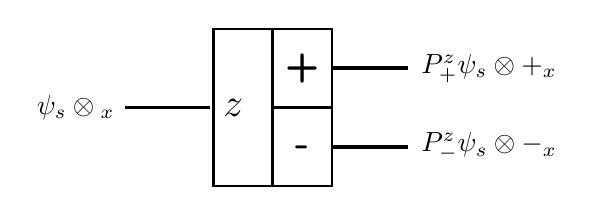
\begin{tikzpicture}[shorten >=1pt,auto, thick,
     square node/.style={rectangle, minimum height=2cm, minimum width=1.50cm, text width = 1.25cm, draw, font=\sffamily\Large\bfseries},
     port/.style={rectangle, draw,  minimum height=1cm, minimum width=0.75cm, font=\sffamily\Large\bfseries},
     wf/.style={rectangle, minimum height=1cm}]
    \apparatus{1}{2}{0}{$z$};

    \node(w0) at (-0.5,0) {$\ket{\psi_s} \otimes \ket{\varnothing_x}$};
    \node[wf] (w1) at (4.75, 0.5) {$P^z_+\ket{\psi_s} \otimes \ket{+_x}$};
    \node[wf] (w2) at (4.75, -0.5) {$P^z_-\ket{\psi_s} \otimes \ket{-_x}$};

    % \node(label1) at (0, -1.75) {$\bm{t_0}$};
    % \node(label2) at (6.25, -1.75) {$\bm{t_1}$};

    \draw[line width=0.5mm] (w0) -- (1);
    \draw[line width=0.5mm] (1+) -- (w1);
    \draw[line width=0.5mm] (1-) -- (w2);
\end{tikzpicture}

\caption[Insert an abbreviated caption here to show in the List of Figures]
{The Stern-Gerlach experiment as described by the von Neumann measurement scheme. Each measurement outcome corresponds to a term in the time-evolved state (\autoref{eq: example 1 final state}). Notice that the measurement interaction results in a branching structure, represented here as a tree graph with the apparatus as a node.}
\label{Figure:Measurement:DetectorStates}
\end{figure}

By describing measurement as a unitary process, we have eliminated many aspects of the quantum measurement problem. However, the interpretation of the final state of the von Neumann measurement scheme comes with its own problems; namely, the preferred basis problem and the problem of outcomes. The problem of outcomes is interpretation dependent, so we address it in TODO ref.

\section{Preferred Basis Problem}

The preferred basis problem arises from the ability to write the final state in \autoref{eq: general final state} using different bases:
\begin{align}
  \ket{\psi_f} = \sum_{n}\left(P^z_n\ket{\psi_s} \otimes \ket{n_x}\right) = \sum_{n'}\left(P^z_{n'}\ket{\psi_s} \otimes \ket{n'_x}\right) =...
\end{align}

\subsection{Example 1}

Consider setting the initial spin state of Example 1 to spin-up in the $x$ direction:
\begin{align}
  \ket{\psi_s} = \ket{+^x_s} = \frac{\ket{+_s} + \ket{-_s}}{\sqrt{2}}
\end{align}

The final state by \autoref{eq: example 1 unitary operator} is
\begin{align}
  \ket{\psi_f} = \frac{\ket{+_s}\otimes\ket{+_x} + \ket{-_s}\otimes\ket{-_x}}{\sqrt{2}}
\end{align}

Similar to the spin system, we can define an orthonormal basis for the position space $\{ \ket{+^x_x}, \ket{-^x_x} \}$:
\begin{align}
  \ket{+^x_x} = \frac{\ket{+_x} + \ket{-_x}}{\sqrt{2}} \\ \nonumber
  \ket{-^x_x} = \frac{\ket{+_x} - \ket{-_x}}{\sqrt{2}}
\end{align}

Then the final state can be written
\begin{align}
  \ket{\psi_f} = \ket{+^x_s} \otimes \ket{+^x_x}
\end{align}

It appears that the measurement process of spin along the $z$ axis resulted in a definite spin state along the $x$ axis. However, as complementary variables, $S_z$ and $S_x$ cannot be simultaneously known. It appears that the von Neumann measurement scheme violates the princple of complementarity. This is the essence of the preferred basis problem.

Without solving this problem, everything works if only the ``right'' questions are asked. We know that we measured spin along the $z$ axis, so we could only ask questions about results in the \textit{preferred basis} (in this case $S_z \otimes x_z$). Rather than ignoring errenous predictions, we can remove them by ensuring that \autoref{eq: general final state} cannot be written in other bases. Such an approach would single out the determination of one variable at an instant of time, incorporating the principle of complementarity directly into the measurement process.

TODO: introduce einselection, inselection.

\section{Inselection}

The von Neumann measurement scheme was originally phrased as the entanglement of a microscopic system with a macroscopic apparatus \cite{Neumann}. Many descriptions of non-unitary Stern-Gerlach measurement consider the electron position state as the state of the apparatus itself. This is a reasonable abstraction, as electron localization is how the state of the apparatus is ``read off''. However, the description it provides is incomplete, because it conflates two distinct physical systems; the apparatus, and the position system belonging to the electron. By labeling the position system as the ``apparatus'', the degree of freedom corresponding to the actual apparatus is effectively ignored.

Newton's third law asserts that the force exerted on the electron by the apparatus magnet is paired with a force exerted on the magnet by the electron. This motivates the definition of apparatus states $\{\ket{+_a}, \ket{-_a}, \ket{\varnothing_a}\}$ representing the effect of positive, negative, and zero torques on the magnet, respectively. Unlike the position states, these states need not be mutually orthongonal. We expect the torque exerted on macroscopic magnets by an electron to be small, so that
\begin{align}
  \braket{n_a | m_a} \approx 1 \neq 1
\end{align}
where $n, m = +, -, \varnothing$. In other words, these states are nearly indistinguishable, but not exactly the same.

We now formalize the spin-position-apparatus interaction, similar to how the implied spin-position correlation in the projection postulate was formalized.
\begin{align} \label{eq: unitary operator inselection}
    \nonumber U(t_1, t_0): \\
    & \ket{\psi} = \left(\sum_{n} P^z_n\ket{\psi_s}\right) \otimes \ket{\varnothing_x} \otimes \ket{\varnothing_a} \mapsto \sum_{n}\left(P^z_n\ket{\psi_s} \otimes \ket{n_x} \otimes \ket{n_a} \right)
\end{align}

While systems in the form \autoref{eq: general final state} do not generally have unique decompositions, systems with three or more components do by the triorthongal decomposition theorem. In other words, we cannot write the final state in another basis:
\begin{align}
  \ket{\psi_f} = \sum_{n}\left(P^z_n\ket{\psi_s} \otimes \ket{n_x} \otimes \ket{n_a} \right) \neq \sum_{n'}\left(P^z_{n'}\ket{\psi_s} \otimes \ket{n'_x} \otimes \ket{n'_a} \right)
\end{align}

Since this is the only possible way to write $\ket{\psi_f}$, the preferred basis has been chosen by just by including the apparatus system. The uniqueness of the decomposition is dependent on the orthogonality of $\ket{n_s}$ states, the orthogonality of $\ket{n_x}$ states, and the non-colinearity of $\ket{n_a}$ states. The apparatus states only need to satisfy $\braket{n_a | m_a} \neq 1$, which is a much looser condition than requiring mutual orthogonality of apparatus states. Misidentifying the position system as the apparatus imposes strict restrictions on the apparatus that truly belong to the position system.

\subsection{Example 1}
Our system is now composed of spin, position, and apparatus systems $H = H_s \otimes H_x \otimes H_a$. The unitary operator satisfying \autoref{eq: unitary operator inselection} is
\begin{align}
  U(t_1, t_0) &= P^z_+ \otimes \left(\: \ket{+_x}\bra{\varnothing_x} \: \bm{+} \: \ket{\varnothing_x}\bra{+_x} \: \bm{+} \: \ket{-_x}\bra{-_x} \: \right) \\ \nonumber
  &\phantom{{}=P^z_+} \otimes \left(\: \ket{+_a}\bra{\varnothing_a} \: \bm{+} \: \ket{\varnothing_a}\bra{+_a} \: \bm{+} \: \ket{-_a}\bra{-_a} \: \right)\\ \nonumber
  &+ P^z_- \otimes \left( \: \ket{-_x}\bra{\varnothing_x} \: \bm{+} \: \ket{\varnothing_x}\bra{-_x} \: \bm{+} \: \ket{+_x}\bra{+_x} \: \right) \\ \nonumber
 &\phantom{{}=P^z_-} \otimes \left(\: \ket{-_a}\bra{\varnothing_a} \: \bm{+} \: \ket{\varnothing_a}\bra{-_a} \: \bm{+} \: \ket{+_a}\bra{+_a} \: \right)
\end{align}

To shorten this expression, we define the ``entanglement operator''
\begin{align}
  E^i_\pm &= \ket{\pm_i}\bra{\varnothing_i} \: \bm{+} \: \ket{\varnothing_i}\bra{\pm_i} \: \bm{+} \: \ket{\mp_i}\bra{\mp_i}
\end{align}

Note that $E$ is Hermitian $\left(E^\dagger = E\right)$ and unitary $\left( E^\dagger E = I \right)$. The unitary operator is now
\begin{align}
  U(t_1, t_0) &= P^z_+ \otimes E^x_+ \otimes E^a_+ \\ \nonumber
  &+ P^z_- \otimes E^x_- \otimes E^a_-
\end{align}

For a general initial spin state, this produces final state
\begin{align}
  \ket{\psi_f} &= P^z_+ \ket{\psi_s} \otimes \ket{+_x} \otimes \ket{+_a} \: \bm{+} \: P^z_- \ket{\psi_s} \otimes \ket{-_x} \otimes \ket{-_a}
\end{align} This experiment is visualized schematically in \autoref{fig: example 1 inselection}.

\begin{figure}
\centering\CaptionFontSize
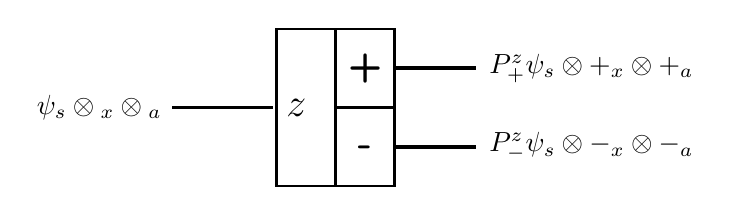
\begin{tikzpicture}[shorten >=1pt,auto, thick,
     square node/.style={rectangle, minimum height=2cm, minimum width=1.50cm, text width = 1.25cm, draw, font=\sffamily\Large\bfseries},
     port/.style={rectangle, draw,  minimum height=1cm, minimum width=0.75cm, font=\sffamily\Large\bfseries},
     wf/.style={rectangle, minimum height=1cm}]
    \apparatus{1}{2}{0}{$z$};

    \node(w0) at (-1,0) {$\ket{\psi_s} \otimes \ket{\varnothing_x} \otimes \ket{\varnothing_a}$};
    \node[wf] (w1) at (5.25, 0.5) {$P^z_+\ket{\psi_s} \otimes \ket{+_x} \otimes \ket{+_a}$};
    \node[wf] (w2) at (5.25, -0.5) {$P^z_-\ket{\psi_s} \otimes \ket{-_x} \otimes \ket{-_a}$};

    % \node(label1) at (0, -1.75) {$\bm{t_0}$};
    % \node(label2) at (6.25, -1.75) {$\bm{t_1}$};

    \draw[line width=0.5mm] (w0) -- (1);
    \draw[line width=0.5mm] (1+) -- (w1);
    \draw[line width=0.5mm] (1-) -- (w2);
\end{tikzpicture}
\caption[Insert an abbreviated caption here to show in the List of Figures]
{The most complete description of Experiment 1 presented, including position and apparatus degres of freedom. The seemingly redundant correlation of both position and apparatus states to spin states makes the abstraction of position states as apparatus states valid. However, formalizing the interaction with the apparatus provides a more complete description that resolves the preferred basis problem.}
\label{fig: example 1 inselection}
\end{figure}

The approach used to solve the preferred basis problem is called \textit{interaction induced superselection} (or \textit{inselection}), since basis selection arises by fully modeling the interaction of the system and the apparatus. A more popular approach is \textit{environment induced superselection} (or \textit{einselection}). It works by the same mechanism, but the third system is the enivornment instead of the apparatus. Since the apparatus is part of the environment in this approach, inselection and einselection are compatible, with inselection providing a more precise description of how the prefered basis is selected. We compare these approaches in greater detail in TODO REF APPENDIX.

The von Neumann measurement scheme can be applied succesivley, on a term-by-term basis, for consecutive measurements. TODO REF details this process for Stern-Gerlach Example 2, and the process is summarized in TODO REF.

\begin{figure}
\centering\CaptionFontSize

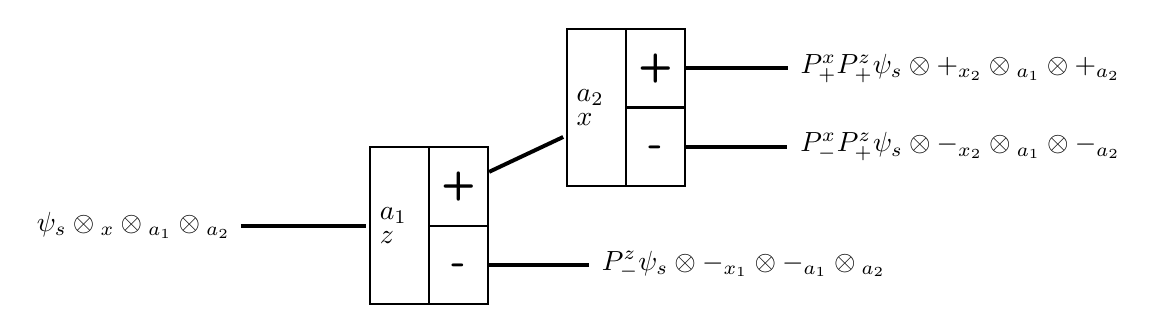
\begin{tikzpicture}[shorten >=1pt,auto, thick,
     square node/.style={rectangle, minimum height=2cm, minimum width=1.50cm, text width = 1.25cm, draw, font=\sffamily\Large\bfseries},
     port/.style={rectangle, draw,  minimum height=1cm, minimum width=0.75cm, font=\sffamily\Large\bfseries},
     wf/.style={rectangle, minimum height=1cm}]
    \apparatus{1}{4}{0}{${}^{a_1}_z$};
    \apparatus{2}{6.5}{1.5}{${}^{a_2}_x$};

    \node(w0) at (0.25,0) {$\ket{\psi_s} \otimes \ket{\varnothing_x} \otimes \ket{\varnothing_{a_1}} \otimes \ket{\varnothing_{a_2}} $};
    \node[wf] (w1) at (8, -.5) {$P^z_-\ket{\psi_s} \otimes \ket{-_{x_1}}  \otimes \ket{-_{a_1}} \otimes \ket{\varnothing_{a_2}}$};
    \node[wf] (w2) at (10.75, 1) {$P^x_-P^z_+\ket{\psi}_s \otimes \ket{-_{x_2}} \otimes \ket{\varnothing_{a_1}} \otimes \ket{-_{a_2}}$};
    \node[wf] (w3) at (10.75, 2) {$P^x_+ P^z_+\ket{\psi_s} \otimes \ket{+_{x_2}} \otimes \ket{\varnothing_{a_1}} \otimes \ket{+_{a_2}}$};

    % \node(label0) at (0, -1.75) {$\bm{t_0}$};
    % \node(label1) at (4.75, -1.75) {$\bm{t_1}$};
    % \node(label2) at (7.25, -1.75) {$\bm{t_2}$};
    % \node(label3) at (9.75, -1.75) {$\bm{t_3}$};
    % \node(bw1) at (-1.75, 1.75) {$P^z_+\ket{\psi}^s \otimes \ket{+}^{D_1}_z \otimes \ket{\varnothing}^{D_2}_x $};

    \draw[line width=0.5mm] (w0) -- (1);
    \draw[line width=0.5mm] (1+) -- (2);
    \draw[line width=0.5mm] (1-) --  (w1);
    \draw[line width=0.5mm] (2+) -- (w3);
    \draw[line width=0.5mm] (2-) -- (w2);


\end{tikzpicture}

\caption[Insert an abbreviated caption here to show in the List of Figures]
{TODO: caption}
\label{Figure:Measurement:labelthis2}
\end{figure}
